\section{back\_\-polygon Class Reference}
\label{classback__polygon}\index{back_polygon@{back\_\-polygon}}
Inheritance diagram for back\_\-polygon:\begin{figure}[H]
\begin{center}
\leavevmode
\includegraphics[width=70pt]{classback__polygon__inherit__graph}
\end{center}
\end{figure}
Collaboration diagram for back\_\-polygon:\begin{figure}[H]
\begin{center}
\leavevmode
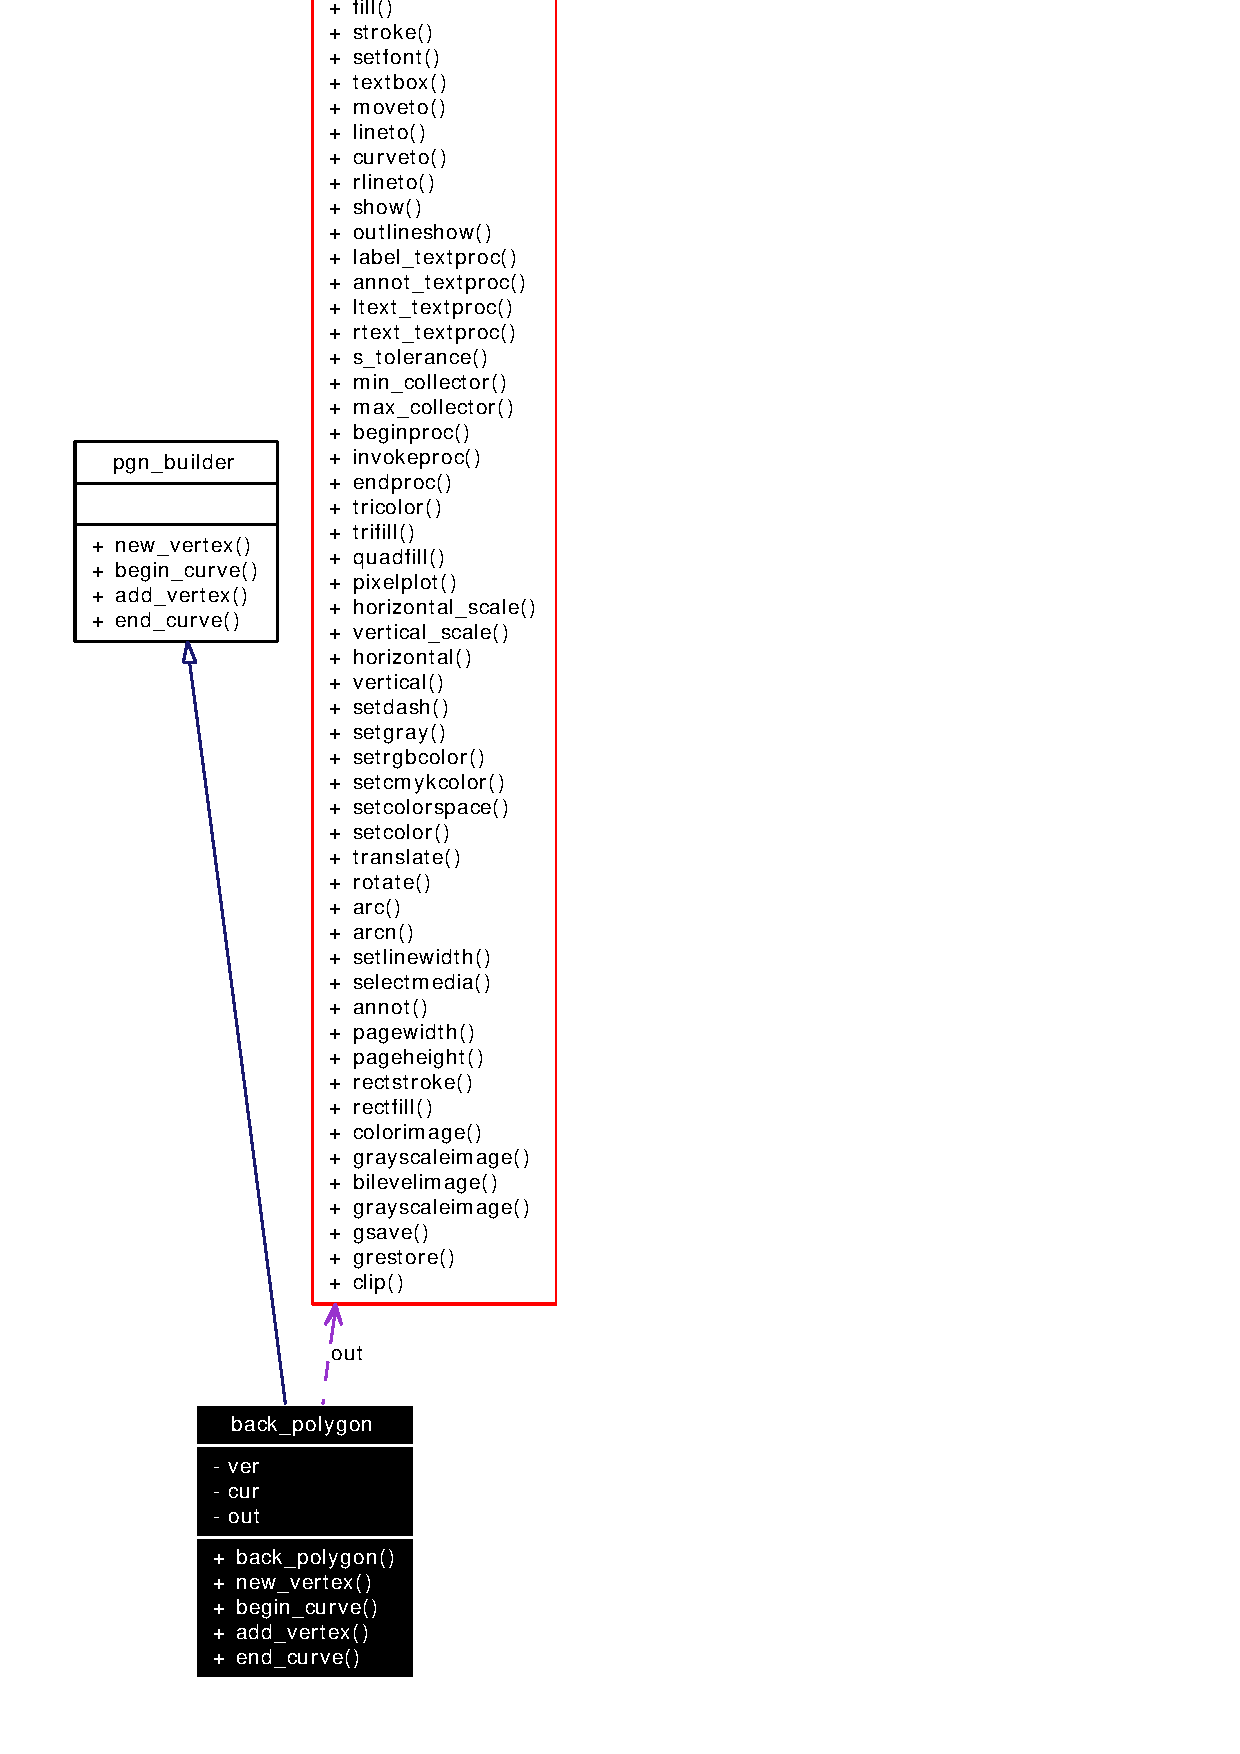
\includegraphics[width=133pt]{classback__polygon__coll__graph}
\end{center}
\end{figure}
\subsection*{Public Member Functions}
\begin{CompactItemize}
\item 
{\bf back\_\-polygon} ({\bf psstream} \&o)\label{classback__polygon_a0}

\item 
int {\bf new\_\-vertex} (double x, double y)\label{classback__polygon_a1}

\item 
void {\bf begin\_\-curve} ()\label{classback__polygon_a2}

\item 
void {\bf add\_\-vertex} (int)\label{classback__polygon_a3}

\item 
void {\bf end\_\-curve} ()\label{classback__polygon_a4}

\end{CompactItemize}


\subsection{Detailed Description}




Definition at line 227 of file ps\_\-data.h.

The documentation for this class was generated from the following files:\begin{CompactItemize}
\item 
ps\_\-data.h\item 
ps\_\-text.cpp\end{CompactItemize}
